% CS615A Aspects of System Administration
% Author: Jan Schaumann <jschauma@netmeister.org>
% $Id: slides.tex,v 1.12 2006/02/12 23:15:03 jschauma Exp $

\special{! TeXDict begin /landplus90{true}store end }

\documentclass[xga]{xdvislides}
\usepackage[landscape]{geometry}
\usepackage{graphics}
\usepackage{graphicx}
\usepackage{colordvi}
\usepackage{tabularx}
\usepackage{multirow}

\newcommand{\gargantuan}{\fontsize{100}{105}\selectfont}

\begin{document}
\setfontphv

%%% Headers and footers
\lhead{\slidetitle}                               % default:\lhead{\slidetitle}
\chead{CS615 - Aspects of System Administration}% default:\chead{\relax}
\rhead{Slide \thepage}                       % default:\rhead{\sectiontitle}
\lfoot{\Gray{Documentation, Multiuser Basics}}% default:\lfoot{\slideauthor}
\cfoot{\relax}                               % default:\cfoot{\relax}
\rfoot{\Gray{\today}}

\vspace*{\fill}
\begin{center}
	\Hugesize
		CS615 - Aspects of System Administration\\ [1em]
		Documentation, Multiuser Basics\\ [1em]
	\hspace*{5mm}\blueline\\ [1em]
	\Normalsize
		Department of Computer Science\\
		Stevens Institute of Technology\\
		Jan Schaumann\\
		\verb+jschauma@stevens.edu+\\
		\verb+http://www.cs.stevens.edu/~jschauma/615/+
\end{center}
\vspace*{\fill}

\subsection{Homework}
Review your submissions.  Ask yourself:
\begin{itemize}
	\item What's the difference in output across operating systems?
	\item What do the different numbers mean?
	\item Why did I open access to port 80?
	\item Why does Solaris mount libc?
	\item Why does {\tt fdisk(8)} claim that {\tt /dev/xvde1 doesn't
		contain a valid partition table}?
	\item Why does Solaris say things like {\tt /dev/dsk/c3d0s0 is
		part of active ZFS pool rpool. Please see zpool(1M).} ?
	\item Why do Solaris partitions show as {\tt unassigned}?
	\item Which partitions are overlapping?  Why?
	\item Do the numbers I produced match?  Do they make sense?
\end{itemize}


\subsection{Last week...}
\begin{center}
	
\includegraphics[scale=0.7]{pics/iran.eps} \\
	{\tt http://is.gd/dUmCk7} \\
	{\tt http://is.gd/rOvsbm}
\end{center}

\subsection{Last week...}
\begin{center}
	
\includegraphics[scale=0.2]{pics/WhitneyHouston.eps} \\
	{\tt http://is.gd/Z7yOgZ} \\
	{\tt http://is.gd/t6NTOy} \\
	{\tt http://is.gd/wWj7TR}
\end{center}

\subsection{Documentation Techniques}
\vfill
\begin{center}
\Huge
Yes, you should write documentation. \\
\small
(Emphasis on either word optional.)
\Normalsize
\end{center}
\vfill

\subsection{Documentation Techniques}
Why?
\begin{itemize}
	\item ``this is: ...''
	\item ``this is why...''
	\item ``this is how...''
	\item ``just so you know...''
	\item ``in case you're interested...''
\end{itemize}

\subsection{Documentation Techniques}
Why?
\begin{itemize}
	\item so you don't forget
	\item so users know how to use the system
	\item so other administrators can repeat what you've done
	\item so {\em you} can repeat what you've done
	\item so you actually do things right
\end{itemize}

\subsection{Documentation Techniques}
Types of documents:

\subsection{Documentation Techniques}
Types of documents:

\begin{itemize}
	\item HOWTO
	\item policies
	\item architecture / design
	\item program documentation / specification
	\item runbook
	\item research
\end{itemize}


\subsection{Documentation Techniques}
Basics:
\begin{itemize}
	\item know your target audience
	\item don't make assumptions
	\item explicitly note your assumptions
	\item include pointers/references to your assumptions
	\item include screen captures where appropriate
	\item include verbatim examples to illustrate common use
\end{itemize}

\subsection{Documentation Techniques}
Documentation is an {\em ongoing} task.

\begin{itemize}
	\item keep track of changes (use a revision control system)
	\item date your documents
\end{itemize}

Documentation is a {\em collaborative} task.

\begin{itemize}
	\item ensure remote access
	\item ensure distributed collaboration
	\item ensure platform/version independence
\end{itemize}


%\subsection{Topics covered}
%A number of multi-user issues, including, but not limited to:
%\\
%
%\begin{itemize}
%	\item technical implications
%	\item user interaction
%	\item politics, policies
%	\item ethical implications
%\end{itemize}
%
%\subsection{Topics covered}
%
%\begin{center}
%	\includegraphics[scale=0.7,angle=-90]{pics/politics.eps}
%\end{center}

\subsection{The meaning of ``{\em multi}user''}
Single user... \\

\begin{center}
	
\includegraphics[scale=0.8]{pics/user.eps}
\end{center}

\subsection{The meaning of ``{\em multi}user''}
Single user... simple causality: \\

\begin{center}
	\includegraphics[scale=1.0]{pics/baseball.eps}
\end{center}

\subsection{The meaning of ``{\em multi}user''}
Many users...

\begin{center}
	
\includegraphics[scale=1.3]{pics/muppets.eps}
\end{center}


\subsection{The meaning of ``{\em multi}user''}
Many users... complex causality:

\begin{center}
	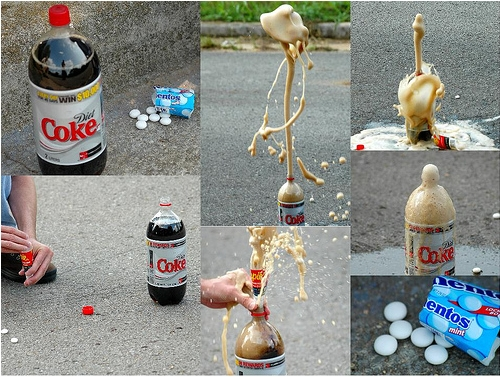
\includegraphics[scale=0.9]{pics/simple-reaction.eps}
\end{center}

\subsection{The meaning of ``{\em multi}user''}
Many users... complex causality:

\begin{center}
	\includegraphics[scale=0.55]{pics/chain-reaction.eps}
\end{center}

\subsection{No more: ``It's mine!''}
\begin{center}
	
\includegraphics[scale=1.0]{pics/gollum.eps}
\end{center}

\subsection{Except, of course, it {\em is} yours.}
\begin{center}
	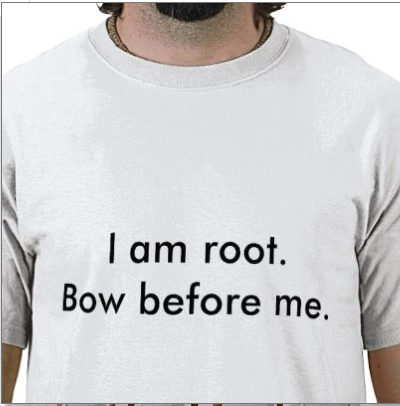
\includegraphics[scale=0.8]{pics/bow-before-me-white.eps}
\end{center}

\subsection{Except, of course, it {\em is} yours.}
\begin{center}
	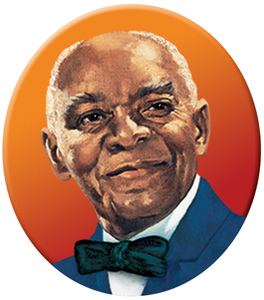
\includegraphics[scale=4.0]{pics/uncle-ben.eps} \\
	\addvspace{.2in}
	\Huge
	``With great power comes great responsibility.''
	\Normalsize
\end{center}

\subsection{Except, of course, it {\em is} yours.}
\begin{center}
	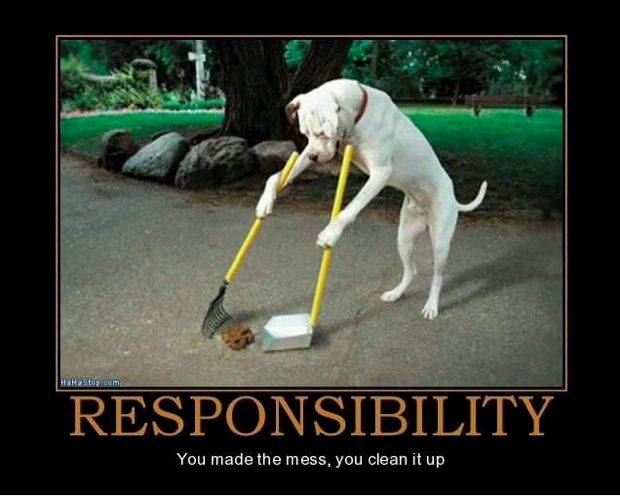
\includegraphics[scale=0.7]{pics/responsibility.eps}
\end{center}


\subsection{Implications of a Multi-User System}
\vspace*{\fill}
\begin{center}
	\includegraphics[scale=0.8]{pics/teamwork.eps}
\end{center}
\vspace*{\fill}

\subsection{Implications of a Multi-User System}
\vspace*{\fill}
\begin{center}
	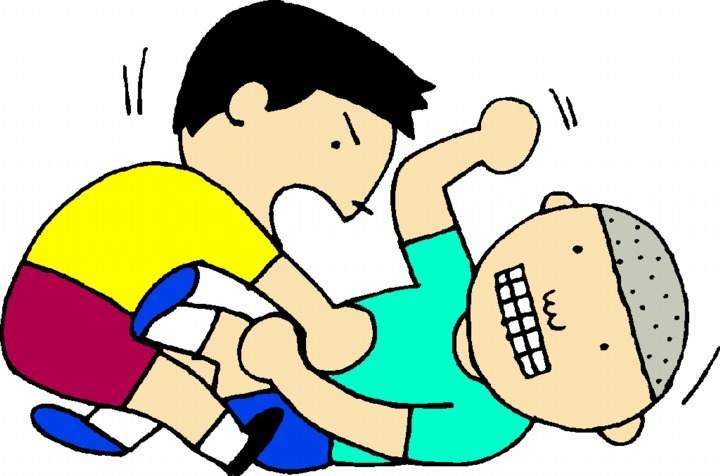
\includegraphics[scale=0.7]{pics/kids_fighting.eps}
\end{center}
\vspace*{\fill}


\subsection{Implications of a Multi-User System}
\vspace*{\fill}
\begin{center}
	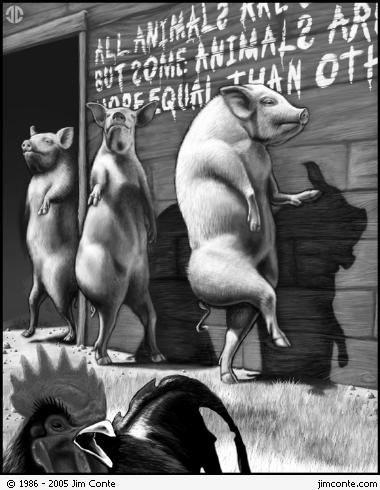
\includegraphics[scale=0.9]{pics/animal_farm.eps}
\end{center}
\vspace*{\fill}

\subsection{Implications of a Multi-User System}
\begin{itemize}
	\item users may want to keep files private
\end{itemize}

\subsection{Implications of a Multi-User System}
\begin{itemize}
	\item users may want to keep files private
	\item users may want to share files
\end{itemize}

\subsection{Implications of a Multi-User System}
\begin{itemize}
	\item users may want to keep files private
	\item users may want to share files
	\item users may (try to gain) access to files they shouldn't have access to
\end{itemize}

\subsection{Implications of a Multi-User System}
\begin{itemize}
	\item users may want to keep files private
	\item users may want to share files
	\item users may (try to gain) access to files they shouldn't have access to
	\item users may (want to) do things that affect other users
\end{itemize}

\subsection{Implications of a Multi-User System}
\begin{itemize}
	\item users may want to keep files private
	\item users may want to share files
	\item users may (try to gain) access to files they shouldn't have access to
	\item users may (want to) do things that affect other users
	\item different users may require different privileges
\end{itemize}

\subsection{Users and User-IDs}
\begin{center}
	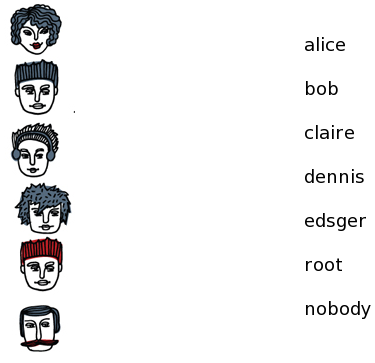
\includegraphics[scale=0.9]{pics/user-sets0.eps} \\
	One-to-one?  Onto?
\end{center}

\subsection{Users and User-IDs}
\begin{center}
	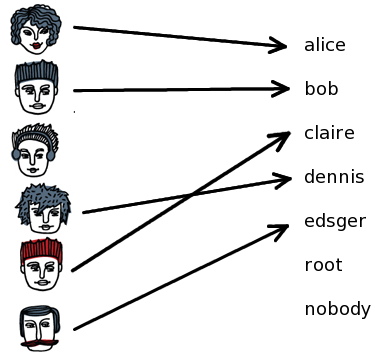
\includegraphics[scale=0.9]{pics/user-sets1.eps} \\
	{\em Not} onto!
\end{center}

\subsection{Users and User-IDs}
\begin{center}
	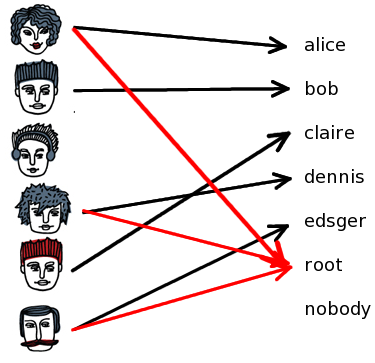
\includegraphics[scale=0.9]{pics/user-sets2.eps} \\
	{\em Not} one-to-one, either!
\end{center}

\subsection{Users and User-IDs}

\begin{center}
	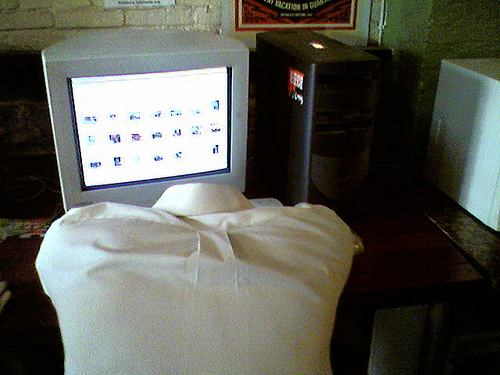
\includegraphics[scale=0.8]{pics/headless.eps} \\
	{\tt nobody}
\end{center}


\subsection{UNIX Fundamentals: User Accounts and File Permissions}
Every account
\begin{itemize}
	\item has a {\em unique} ID
	\item belongs to at least one group
	\item may or may not be password protected
	\item may or may not have a valid login program
\end{itemize}

\subsection{UNIX Fundamentals: User Accounts and File Permissions}
Every account
\begin{itemize}
	\item has a {\em unique} ID
	\item belongs to at least one group
	\item may or may not be password protected
	\item may or may not have a valid login program
\end{itemize}
\addvspace{.5in}
Every file
\begin{itemize}
	\item is associated with a {\em uid} and a {\em gid}
	\item has a number of protection bits
\end{itemize}


\subsection{Unix Groups}
\begin{itemize}
	\item enables {\em arbitrary} collections of users to share resources
	\item information stored in \verb+/etc/group+, format is: \\
		\verb+name:*:GID:user1,user2,...+
	\item most Unix systems impose a limit of 16 or 32 group memberships per
		user
	\item most Unix systems have a common default group for new users (some
		Linux versions deviate)
	\item some Unix systems have group shadow files
\end{itemize}

\subsection{UNIX Fundamentals: User Accounts and File Permissions}
Example:
\begin{verbatim}
$ ls -Tail
total 4688
436334 drwx------  2 jschauma  wheel      512 Feb  8 15:36:53 2004 .
436224 drwxrwxrwt  6 root      wheel      512 Feb  8 15:29:01 2004 ..
436314 crw-------  1 root      wheel     1, 2 Feb  8 15:31:00 2004 bar
436317 brw-r--r--  1 root      wheel     2, 3 Feb  8 15:31:27 2004 baz
436321 -rw-------  2 jschauma  users     7360 Feb  8 15:32:58 2004 blafasel
436319 lrwx------  1 jschauma  wheel        1 Feb  8 15:32:20 2004 blah -> n
436321 -rw-------  2 jschauma  users     7360 Feb  8 15:32:58 2004 fofo
436311 prw-------  1 jschauma  wheel        0 Feb  8 15:28:32 2004 foo
     4 -rwxr-sr-x  2 root      wheel  2344675 Jan 22 12:41:10 2004 garg
$
\end{verbatim}

\subsection{Consider Scalability}
Things to consider:
\\

\begin{center}
	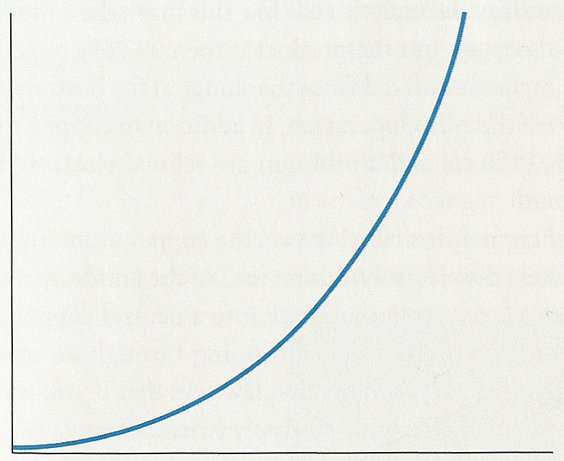
\includegraphics[scale=2.8]{pics/exponential_growth.eps}
\end{center}

\subsection{Consider Scalability}
Things to consider:
\\

\begin{center}
	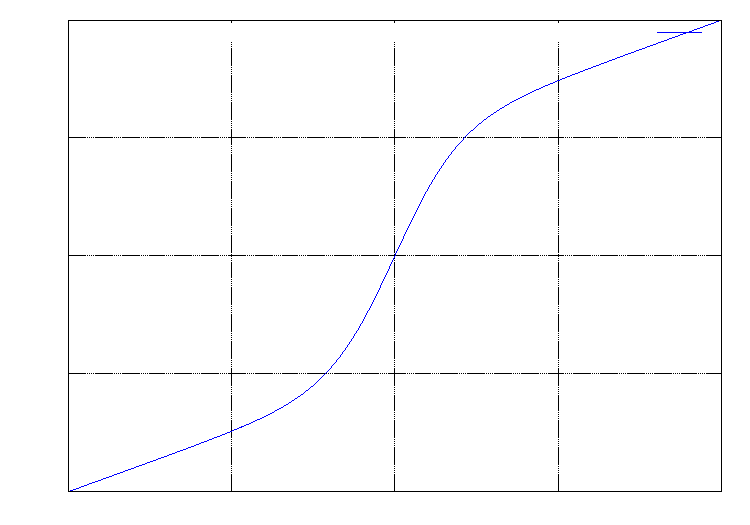
\includegraphics[scale=0.8]{pics/hyperbolic_tangent.eps}
\end{center}

\subsection{Adding and Removing Accounts}
\begin{center}
	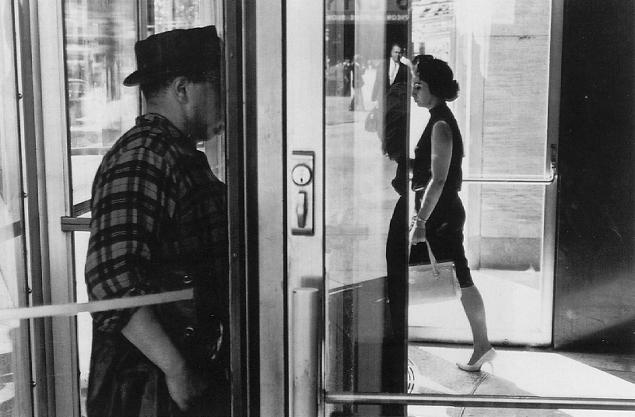
\includegraphics[scale=0.8]{pics/friedlander_revolving_door.eps}
\end{center}



\subsection{Adding accounts}
Things to consider:
\begin{itemize}
	\item create/assign username, UID, primary group, supplementary groups,
		choose shell
\end{itemize}

\subsection{Adding accounts}
Things to consider:
\begin{itemize}
	\item create/assign username, UID, primary group, supplementary groups,
		choose shell
	\item assign a password
\end{itemize}

\subsection{Adding accounts}
Things to consider:
\begin{itemize}
	\item create/assign username, UID, primary group, supplementary groups,
		choose shell
	\item assign a password
	\item create a home directory
\end{itemize}

\subsection{Adding accounts}
Things to consider:
\begin{itemize}
	\item create/assign username, UID, primary group, supplementary groups,
		choose shell
	\item assign a password
	\item create a home directory
	\item place initialialization files in the user's home directory
\end{itemize}

\subsection{Adding accounts}
Things to consider:
\begin{itemize}
	\item create/assign username, UID, primary group, supplementary groups,
		choose shell
	\item assign a password
	\item create a home directory
	\item place initialialization files in the user's home directory
	\item set other parameters (password aging, resource limits...)
\end{itemize}

\subsection{Adding accounts}
Things to consider:
\begin{itemize}
	\item create/assign username, UID, primary group, supplementary groups,
		choose shell
	\item assign a password
	\item create a home directory
	\item place initialialization files in the user's home directory
	\item set other parameters (password aging, resource limits...)
	\item add user to other facilities (enable disk quota, mail filters,
		printer subsystem...)
\end{itemize}

\subsection{Adding accounts}
Things to consider:
\begin{itemize}
	\item create/assign username, UID, primary group, supplementary groups,
		choose shell
	\item assign a password
	\item create a home directory
	\item place initialialization files in the user's home directory
	\item set other parameters (password aging, resource limits...)
	\item add user to other facilities (enable disk quota, mail filters,
		printer subsystem...)
	\item perform any other site-specific initialization tasks
\end{itemize}

\subsection{Disabling and Removing User Accounts}
Things to consider:
\begin{itemize}
	\item change other passwords
\end{itemize}

\subsection{Disabling and Removing User Accounts}
Things to consider:
\begin{itemize}
	\item change other passwords
	\item terminate running processes
\end{itemize}

\subsection{Disabling and Removing User Accounts}
Things to consider:
\begin{itemize}
	\item change other passwords
	\item terminate running processes
	\item remove user from secondary groups
\end{itemize}

\subsection{Disabling and Removing User Accounts}
Things to consider:
\begin{itemize}
	\item change other passwords
	\item terminate running processes
	\item remove user from secondary groups
	\item (re)define a mail alias or redirect mail
\end{itemize}

\subsection{Disabling and Removing User Accounts}
Things to consider:
\begin{itemize}
	\item change other passwords
	\item terminate running processes
	\item remove user from secondary groups
	\item (re)define a mail alias or redirect mail
	\item remove any cronjobs or other pending tasks for that user
\end{itemize}

\subsection{Disabling and Removing User Accounts}
Things to consider:
\begin{itemize}
	\item change other passwords
	\item terminate running processes
	\item remove user from secondary groups
	\item (re)define a mail alias or redirect mail
	\item remove any cronjobs or other pending tasks for that user
	\item backup all of the users files
\end{itemize}

\subsection{Disabling and Removing User Accounts}
Things to consider:
\begin{itemize}
	\item change other passwords
	\item terminate running processes
	\item remove user from secondary groups
	\item (re)define a mail alias or redirect mail
	\item remove any cronjobs or other pending tasks for that user
	\item backup all of the users files
	\item perform any other site-specific tasks
\end{itemize}

\subsection{Practical Policies}

\begin{center}
	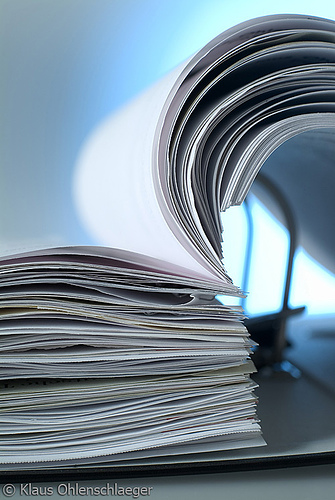
\includegraphics[scale=0.7]{pics/documents.eps}
\end{center}

\subsection{Practical Policies}
Some important policy documents you may need:
\begin{itemize}
	\item service level agreements (SLAs) for routine tasks
	\item administrative service policies
	\item rights and responsibilities of users
	\item policies regarding sysadmin or other users with special
		privileges
	\item guest account policies
	\item disaster recovery plan
	\item security incidence response plan
	\item software licensing (inbound, in-house, outbound)
	\item ...
\end{itemize}

\subsection{Software Licensing}
\begin{itemize}
	\item Operating Systems
	\item Commercial Closed Source Software
	\item Open Source Software
	\item In-House Usage as well as outside the organization
	\item Installation of software
\end{itemize}
\addvspace{.5in}
Read and understand all licenses for software you install!


\subsection{Practical Policies}
\begin{center}
	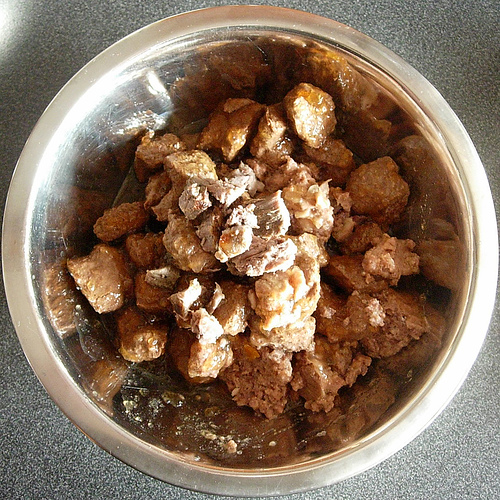
\includegraphics[scale=0.9]{pics/dogfood.eps}
\end{center}

\subsection{Policy Enforcement}
In order to enforce a policy you need to make sure, that
\begin{itemize}
	\item all involved parties are informed of the policy
\end{itemize}

\subsection{Policy Enforcement}
In order to enforce a policy you need to make sure, that
\begin{itemize}
	\item all involved parties are informed of the policy
	\item you log relevant information
\end{itemize}

\subsection{Policy Enforcement}
In order to enforce a policy you need to make sure, that
\begin{itemize}
	\item all involved parties are informed of the policy
	\item you log relevant information
	\item logs cannot be tempered with and are secure
\end{itemize}

\subsection{Policy Enforcement}
In order to enforce a policy you need to make sure, that
\begin{itemize}
	\item all involved parties are informed of the policy
	\item you log relevant information
	\item logs cannot be tempered with and are secure
	\item you have buy-in from all stakeholders
\end{itemize}

\subsection{Ethics}

\begin{center}
	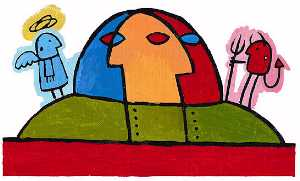
\includegraphics[scale=2.5]{pics/angel-devil.eps}
\end{center}


\subsection{Ethics}
The SAGE Code of Ethics:
\\

\newcolumntype{S}{>{\centering\arraybackslash} m{.4\linewidth} }
\begin{tabular}{ p{10cm} S }
\begin{itemize}
	\item Professionalism
\end{itemize}
& \multirow{20}{*}{
\includegraphics[scale=1.3]{pics/angel.eps}} \\
\end{tabular}

\subsection{Ethics}
The SAGE Code of Ethics:
\\

\begin{tabular}{ p{10cm} S }
\begin{itemize}
	\item Professionalism
	\item Personal Integrity
\end{itemize}
& \multirow{20}{*}{
\includegraphics[scale=1.3]{pics/angel.eps}} \\
\end{tabular}

\subsection{Ethics}
The SAGE Code of Ethics:
\\

\begin{tabular}{ p{10cm} S }
\begin{itemize}
	\item Professionalism
	\item Personal Integrity
	\item Privacy
\end{itemize}
& \multirow{20}{*}{
\includegraphics[scale=1.3]{pics/angel.eps}} \\
\end{tabular}

\subsection{Ethics}
The SAGE Code of Ethics:
\\

\begin{tabular}{ p{10cm} S }
\begin{itemize}
	\item Professionalism
	\item Personal Integrity
	\item Privacy
	\item Laws and Policies
\end{itemize}
& \multirow{20}{*}{
\includegraphics[scale=1.3]{pics/angel.eps}} \\
\end{tabular}


\subsection{Ethics}
The SAGE Code of Ethics:
\\

\begin{tabular}{ p{10cm} S }
\begin{itemize}
	\item Professionalism
	\item Personal Integrity
	\item Privacy
	\item Laws and Policies
	\item System Integrity
\end{itemize}
& \multirow{20}{*}{
\includegraphics[scale=1.3]{pics/angel.eps}} \\
\end{tabular}


\subsection{Ethics}
The SAGE Code of Ethics:
\\

\begin{tabular}{ p{10cm} S }
\begin{itemize}
	\item Professionalism
	\item Personal Integrity
	\item Privacy
	\item Laws and Policies
	\item System Integrity
	\item Education
\end{itemize}
& \multirow{20}{*}{
\includegraphics[scale=1.3]{pics/angel.eps}} \\
\end{tabular}


\subsection{Ethics}
The SAGE Code of Ethics:
\\

\begin{tabular}{ p{10cm} S }
\begin{itemize}
	\item Professionalism
	\item Personal Integrity
	\item Privacy
	\item Laws and Policies
	\item System Integrity
	\item Education
	\item Social Responsibility
\end{itemize}
& \multirow{20}{*}{
\includegraphics[scale=1.3]{pics/angel.eps}} \\
\end{tabular}


\subsection{Ethics}
The SAGE Code of Ethics:
\\

\begin{tabular}{ p{10cm} S }
\begin{itemize}
	\item Professionalism
	\item Personal Integrity
	\item Privacy
	\item Laws and Policies
	\item System Integrity
	\item Education
	\item Social Responsibility
	\item Ethical Responsibility
\end{itemize}
& \multirow{20}{*}{
\includegraphics[scale=1.3]{pics/angel.eps}} \\
\end{tabular}


%\subsection{Examples}
%A number of random examples on more or less complicated ethical matters:
%\\
%
%\begin{tabular}{ p{12cm} S }
%\begin{itemize}
%	\item objectionable website content
%\end{itemize}
%& \multirow{20}{*}{\includegraphics[scale=1.3]{pics/devil.eps}} \\
%\end{tabular}
%
%\subsection{Examples}
%A number of random examples on more or less complicated ethical matters:
%\\
%
%\begin{tabular}{ p{12cm} S }
%\begin{itemize}
%	\item objectionable website content
%	\item manipulating other users' email
%\end{itemize}
%& \multirow{20}{*}{\includegraphics[scale=1.3]{pics/devil.eps}} \\
%\end{tabular}
%
%\subsection{Examples}
%A number of random examples on more or less complicated ethical matters:
%\\
%
%\begin{tabular}{ p{12cm} S }
%\begin{itemize}
%	\item objectionable website content
%	\item manipulating other users' email
%	\item granting others access
%\end{itemize}
%& \multirow{20}{*}{\includegraphics[scale=1.3]{pics/devil.eps}} \\
%\end{tabular}
%
%\subsection{Examples}
%A number of random examples on more or less complicated ethical matters:
%\\
%
%\begin{tabular}{ p{12cm} S }
%\begin{itemize}
%	\item objectionable website content
%	\item manipulating other users' email
%	\item granting others access
%	\item dealing with law enforcement
%\end{itemize}
%& \multirow{20}{*}{\includegraphics[scale=1.3]{pics/devil.eps}} \\
%\end{tabular}
%
%\subsection{Examples}
%A number of random examples on more or less complicated ethical matters:
%\\
%
%\begin{tabular}{ p{12cm} S }
%\begin{itemize}
%	\item objectionable website content
%	\item manipulating other users' email
%	\item granting others access
%	\item dealing with law enforcement
%	\item following orders / following local law
%\end{itemize}
%& \multirow{20}{*}{\includegraphics[scale=1.3]{pics/devil.eps}} \\
%\end{tabular}
%

\subsection{At the end of the day...}
\begin{center}
	
\includegraphics[scale=0.5]{pics/thumbsup-borat.eps}
\end{center}

\subsection{Reading}
User Management:
\begin{itemize}
	\item {\em Frisch}: Ch 6; {\em Burgess}: Ch 5;
	\item \verb+passwd(5)+, \verb+passwd.conf(5)+, \verb+login.conf(5)+,
		\verb+vipw(8)+
	\item \verb+group(5)+
	\item \verb+useradd(8)+, \verb+usermod(8)+, \verb+user(8)+,
		\verb+usermgmt.conf(5)+
	\item \verb+userdel(8)+
\end{itemize}
Ethics:
\begin{itemize}
	\item \verb+http://www.sage.org/ethics/+
	\item \verb+http://www.acm.org/about/code-of-ethics+
\end{itemize}

\subsection{Reading}
Licenses:
\begin{itemize}
	\item \verb+http://www.opensource.org/licenses/+
	\item \verb+http://www.netbsd.org/about/redistribution.html+
	\item \verb+http://www.gnu.org/licenses/licenses.html+
	\item \verb+http://java.sun.com/j2se/1.5.0/scsl_5.0-license.txt+
	\item \verb+http://faqs.org/faqs/law/copyright/faq/+
\end{itemize}

\subsection{Professional Organizations}
\begin{itemize}
	\item \verb+http://www.usenix.org/+ and \verb+http://www.sage.org/+
	\item \verb+http://www.lopsa.org/+
	\item \verb+http://www.acm.org/+
	\item \verb+http://www.isoc.org/+
	\item \verb+http://www.nanog.org/+
\end{itemize}

\end{document}
